\section{Specimen \circled{1} : Michael-Scott queue}

% ---------------------------------------------------------

\begin{frame}{Original algorithm (1996)}
\centering
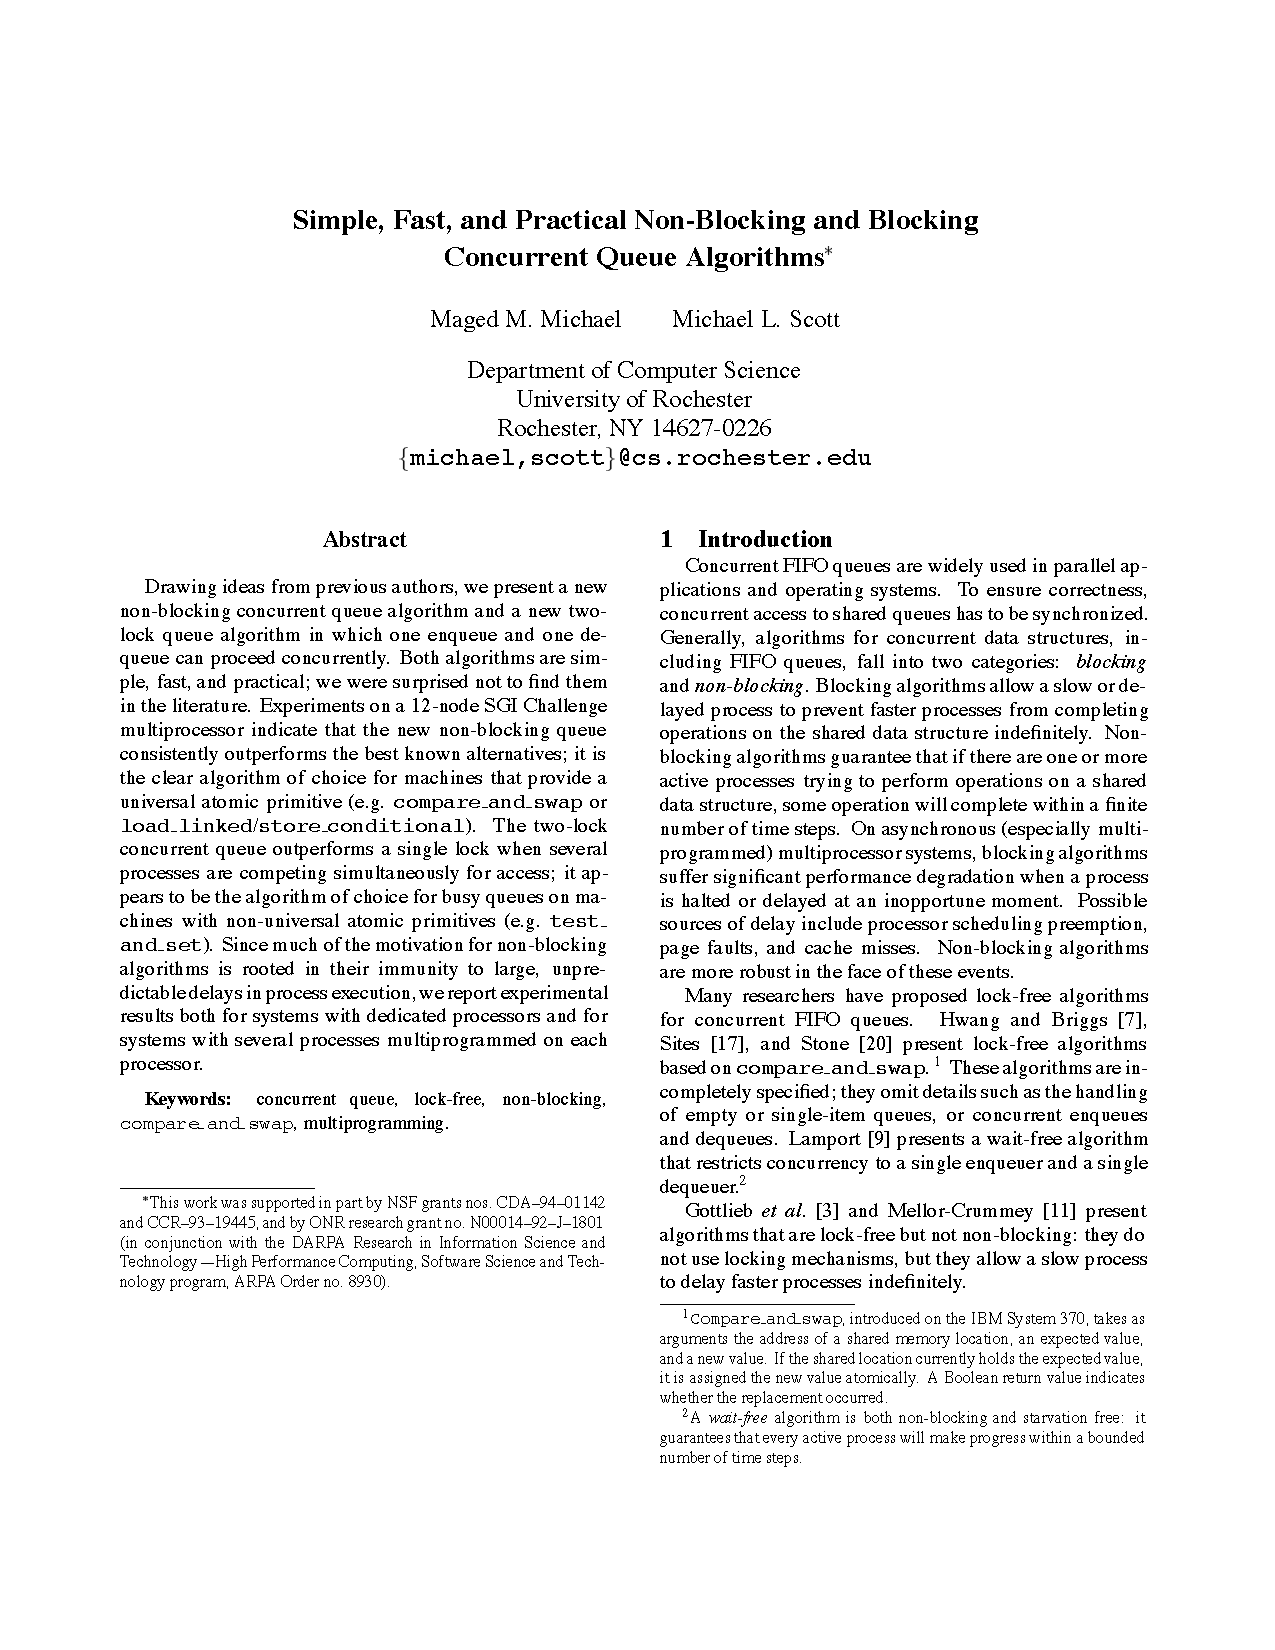
\includegraphics[scale=0.5]{images/michael_scott_1996.pdf}
\end{frame}

% ---------------------------------------------------------

\begin{frame}{Basic implementation}
\begin{adjustwidth}{-1em}{-1em}
\centering
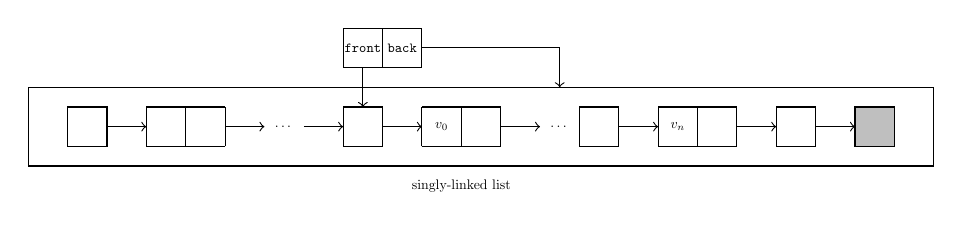
\begin{tikzpicture}[scale=0.5, every node/.style={scale=0.5}]
    \draw (0,0) rectangle ++(1,1) ;
    \draw [->] (1,0.5) -- ++(1,0) ;
    \draw (2,0) grid ++(2,1) ;
    \draw [->] (4,0.5) -- ++(1,0) ;
    \node at (5.5,0.5) {\ldots} ;
    \draw [->] (6,0.5) -- ++(1,0) ;
    \draw (7,0) rectangle ++(1,1) ;
    \draw [->] (8,0.5) -- ++(1,0) ;
    \draw (9,0) grid ++(2,1) ;
    \node at (9.5,0.5) {$v_0$} ;
    \draw [->] (11,0.5) -- ++(1,0) ;
    \node at (12.5,0.5) {\ldots} ;
    \draw (13,0) rectangle ++ (1,1) ;
    \draw [->] (14,0.5) -- ++(1,0) ;
    \draw (15,0) grid ++(2,1) ;
    \node at (15.5,0.5) {$v_n$} ;
    \draw [->] (17,0.5) -- ++(1,0) ;
    \draw (18,0) rectangle ++(1,1) ;
    \draw [->] (19,0.5) -- ++(1,0) ;
    \draw [fill=lightgray] (20,0) rectangle ++(1,1) ;
    
    \draw (-1,-0.5) rectangle ++(23,2) ;
    \node at (10,-1) {singly-linked list} ;
    
    \draw (7,2) grid ++(2,1) ;
    \draw [->] (7.5,2) -- ++(0,-1) ;
    \draw [->] (9,2.5) -| ++(3.5,-1) ;
    \node at (7.5,2.5) {\texttt{front}} ;
    \node at (8.5,2.5) {\texttt{back}} ;
\end{tikzpicture}
\vfill
\begin{itemize}
    \item The queue contains $[v_0, \cdots, v_n]$.
    \item \texttt{front} points to the first component of the active part of the list.
    \item \texttt{back} points somewhere in the list, usually closer to the end.
\end{itemize}
\end{adjustwidth}
\end{frame}

% ---------------------------------------------------------

\begin{frame}{\texttt{push} linearization}
\begin{adjustwidth}{-1em}{-1em}
\centering
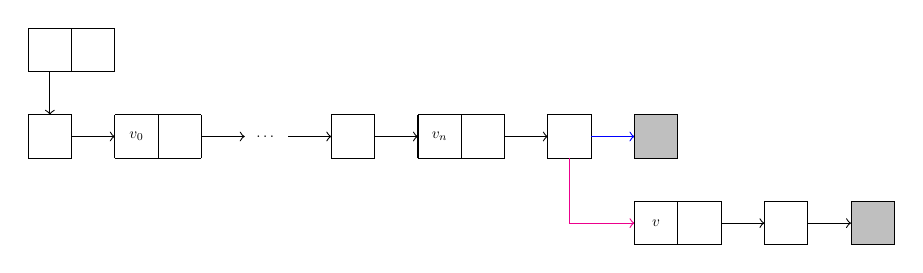
\begin{tikzpicture}[scale=0.55, every node/.style={scale=0.55}]
    \draw (0,0) rectangle ++(1,1) ;
    \draw [->] (1,0.5) -- ++(1,0) ;
    \draw (2,0) grid ++(2,1) ;
    \node at (2.5,0.5) {$v_0$} ;
    \draw [->] (4,0.5) -- ++(1,0) ;
    \node at (5.5,0.5) {\ldots} ;
    \draw [->] (6, 0.5) -- ++(1,0) ;
    \draw (7,0) rectangle ++ (1,1) ;
    \draw [->] (8,0.5) -- ++(1,0) ;
    \draw (9,0) grid ++(2,1) ;
    \node at (9.5,0.5) {$v_n$} ;
    \draw [->] (11,0.5) -- ++(1,0) ;
    \draw (12,0) rectangle ++(1,1) ;
    \draw [->, blue] (13,0.5) -- ++(1,0) ;
    \draw [fill=lightgray] (14,0) rectangle ++(1,1) ;
    \draw [->, magenta] (12.5,0) |- ++(1.5,-1.5) ;
    \draw (14,-2) grid ++(2,1) ;
    \node at (14.5,-1.5) {$v$} ;
    \draw [->] (16,-1.5) -- ++(1,0) ;
    \draw (17,-2) rectangle ++(1,1) ;
    \draw [->] (18,-1.5) -- ++(1,0) ;
    \draw [fill=lightgray] (19,-2) rectangle ++(1,1) ;
    
    \draw (0,2) grid ++(2,1) ;
    \draw [->] (0.5,2) -- ++(0,-1) ;
\end{tikzpicture}
\vfill
\begin{tabular}{c}
        $\mathrm{queue \mathhyphen model}\ t\ [v_0, \cdots, v_n]$
    \\
        $\Downarrow$
    \\
        $\mathrm{queue \mathhyphen model}\ t\ [v_0, \cdots, v_n, v]$
\end{tabular}
\end{adjustwidth}
\end{frame}

% ---------------------------------------------------------

\begin{frame}{\texttt{pop} linearization}
\begin{adjustwidth}{-1em}{-1em}
\centering
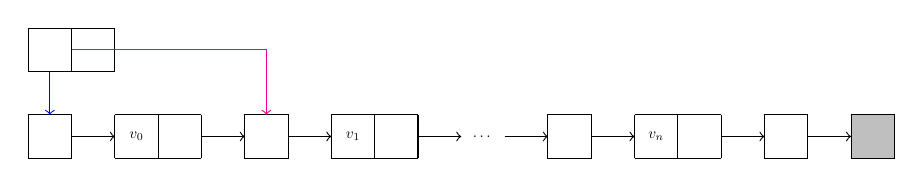
\begin{tikzpicture}[scale=0.55, every node/.style={scale=0.55}]
    \draw (0,0) rectangle ++(1,1) ;
    \draw [->] (1,0.5) -- ++(1,0) ;
    \draw (2,0) grid ++(2,1) ;
    \node at (2.5,0.5) {$v_0$} ;
    \draw [->] (4,0.5) -- ++(1,0) ;
    \draw (5,0) rectangle ++(1,1) ;
    \draw [->] (6,0.5) -- ++(1,0) ;
    \draw (7,0) grid ++(2,1) ;
    \node at (7.5,0.5) {$v_1$} ;
    \draw [->] (9,0.5) -- ++(1,0) ;
    \node at (10.5,0.5) {\ldots} ;
    \draw [->] (11, 0.5) -- ++(1,0) ;
    \draw (12,0) rectangle ++ (1,1) ;
    \draw [->] (13,0.5) -- ++(1,0) ;
    \draw (14,0) grid ++(2,1) ;
    \node at (14.5,0.5) {$v_n$} ;
    \draw [->] (16,0.5) -- ++(1,0) ;
    \draw (17,0) rectangle ++(1,1) ;
    \draw [->] (18,0.5) -- ++(1,0) ;
    \draw [fill=lightgray] (19,0) rectangle ++(1,1) ;
    
    \draw (0,2) grid ++(2,1) ;
    \draw [->, blue] (0.5,2) -- ++(0,-1) ;
    \draw [->, magenta] (1,2.5) -| ++(4.5,-1.5) ;
\end{tikzpicture}
\vfill
\begin{tabular}{c}
        $\mathrm{queue \mathhyphen model}\ t\ [v_0, \cdots, v_n]$
    \\
        $\Downarrow$
    \\
        $\mathrm{queue \mathhyphen model}\ t\ [v_1, \cdots, v_n]$
\end{tabular}
\end{adjustwidth}
\end{frame}

% ---------------------------------------------------------

\begin{frame}[fragile]{Basic \OCaml~5 implementation}
\begin{minted}{ocaml}
type 'a node =
  | Nil
  | Next of 'a * 'a node Atomic.t

type 'a t = {
  front: 'a node Atomic.t Atomic.t ;
  back: 'a node Atomic.t Atomic.t ;
}
\end{minted}
\end{frame}

% ---------------------------------------------------------

\begin{frame}{Specification}
\large
\[
  \aspec{
    \mathcolor{cyan}{\mathrm{queue \mathhyphen inv}}\ t\ \iota
  }{
    \mathit{vs}
  }{
    \mathcolor{orange}{\mathrm{queue \mathhyphen model}}\ t\ \mathit{vs}
  }{
    \texttt{queue\_push}\ t\ v,\ \uparrow \iota
  }{
    \mathcolor{orange}{\mathrm{queue \mathhyphen model}}\ t\ (\mathit{vs} \mdoubleplus [v])
  }{
    \texttt{()}
  }{
    \iTrue
  }
\]
\vfill
\[
  \aspec{
    \mathcolor{cyan}{\mathrm{queue \mathhyphen inv}}\ t\ \iota
  }{
    \mathit{vs}
  }{
    \mathcolor{orange}{\mathrm{queue \mathhyphen model}}\ t\ \mathit{vs}
  }{
    \texttt{queue\_pop}\ t,\ \uparrow \iota
  }{
    \mathcolor{orange}{\mathrm{queue \mathhyphen model}}\ t\ (\mathrm{tail}\ \mathit{vs})
  }{
    \mathrm{head}\ \mathit{vs}
  }{
    \iTrue
  }
\]
\end{frame}

% ---------------------------------------------------------

\begin{frame}{Verification by Vindum \& Birkedal (2021)}
\centering

\includegraphics[scale=0.5]{images/vindum_birkedal_2021.pdf}
\begin{overbox}<2>
    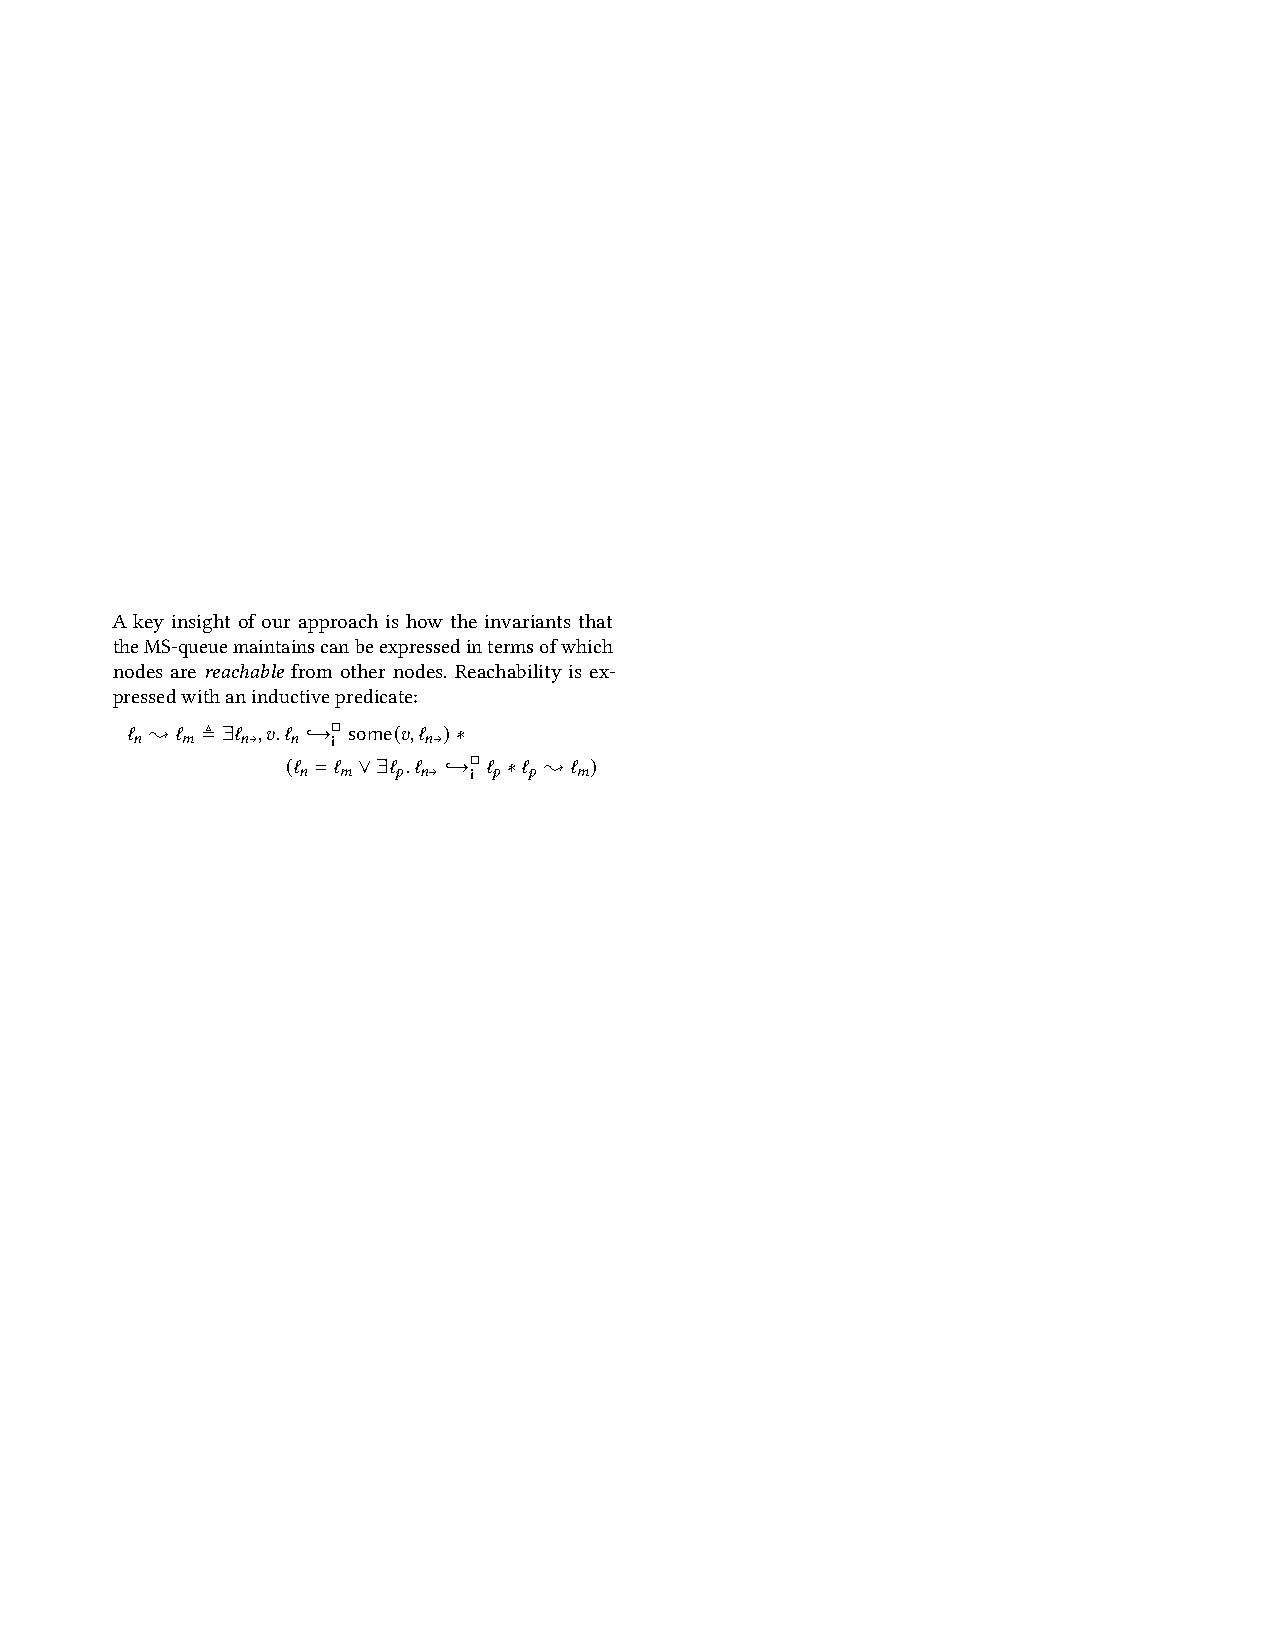
\includegraphics{images/vindum_birkedal_2021_excerpt.pdf}
\end{overbox}
\end{frame}

% ---------------------------------------------------------

\begin{frame}{Optimized implementation}
\begin{adjustwidth}{-1em}{-1em}
\centering
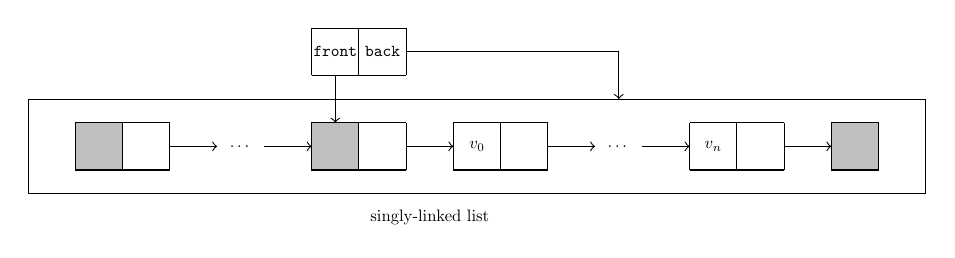
\begin{tikzpicture}[scale=0.6, every node/.style={scale=0.6}]
    \draw (0,0) grid ++(2,1) ;
    \draw [fill=lightgray] (0,0) rectangle ++(1,1) ;
    \draw [->] (2,0.5) -- ++(1,0) ;
    \node at (3.5,0.5) {\ldots} ;
    \draw [->] (4,0.5) -- ++(1,0) ;
    \draw (5,0) grid ++(2,1) ;
    \draw [fill=lightgray] (5,0) rectangle ++(1,1) ;
    \draw [->] (7,0.5) -- ++(1,0) ;
    \draw (8,0) grid ++(2,1) ;
    \node at (8.5,0.5) {$v_0$} ;
    \draw [->] (10, 0.5) -- ++(1,0) ;
    \node at (11.5,0.5) {\ldots} ;
    \draw [->] (12,0.5) -- ++(1,0) ;
    \draw (13,0) grid ++(2,1) ;
    \node at (13.5,0.5) {$v_n$} ;
    \draw [->] (15,0.5) -- ++(1,0) ;
    \draw [fill=lightgray] (16,0) rectangle ++(1,1) ;
    
    \draw (-1,-0.5) rectangle ++(19,2) ;
    \node at (7.5,-1) {singly-linked list} ;
    
    \draw (5,2) grid ++(2,1) ;
    \draw [->] (5.5,2) -- ++(0,-1) ;
    \draw [->] (7,2.5) -| ++(4.5,-1) ;
    \node at (5.5,2.5) {\texttt{front}} ;
    \node at (6.5,2.5) {\texttt{back}} ;
\end{tikzpicture}
\vfill
\begin{itemize}
    \item The queue contains $[v_0, \cdots, v_n]$.
    \item \texttt{front} points to the first component of the active part of the list.
    \item \texttt{back} points somewhere in the list, usually closer to the end.
\end{itemize}
\end{adjustwidth}
\end{frame}

% ---------------------------------------------------------

\begin{frame}{\texttt{push} linearization}
\begin{adjustwidth}{-1em}{-1em}
\centering
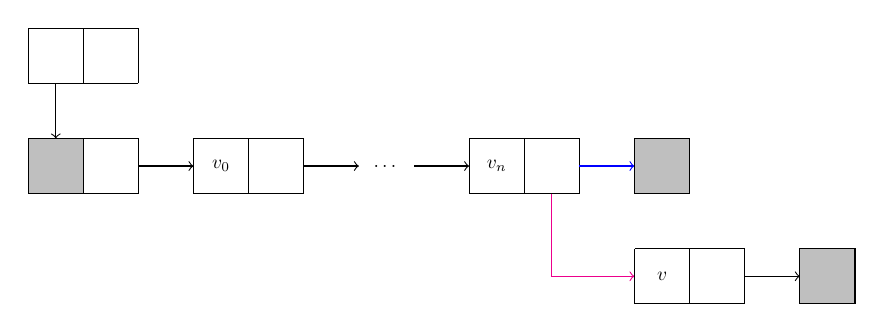
\begin{tikzpicture}[scale=0.7, every node/.style={scale=0.7}]
    \draw (0,0) grid ++(2,1) ;
    \draw [fill=lightgray] (0,0) rectangle ++(1,1) ;
    \draw [->] (2,0.5) -- ++(1,0) ;
    \draw (3,0) grid ++(2,1) ;
    \node at (3.5,0.5) {$v_0$} ;
    \draw [->] (5,0.5) -- ++(1,0) ;
    \node at (6.5,0.5) {\ldots} ;
    \draw [->] (7,0.5) -- ++(1,0) ;
    \draw (8,0) grid ++(2,1) ;
    \node at (8.5,0.5) {$v_n$} ;
    \draw [->, blue] (10,0.5) -- ++(1,0) ;
    \draw [fill=lightgray] (11,0) rectangle ++(1,1) ;
    \draw [->, magenta] (9.5,0) |- ++(1.5,-1.5) ;
    \draw (11,-2) grid ++(2,1) ;
    \node at (11.5,-1.5) {$v$} ;
    \draw [->] (13,-1.5) -- ++(1,0) ;
    \draw [fill=lightgray] (14,-2) rectangle ++(1,1) ;
    
    \draw (0,2) grid ++(2,1) ;
    \draw [->] (0.5,2) -- ++(0,-1) ;
\end{tikzpicture}
\vfill
\begin{tabular}{c}
        $\mathrm{queue \mathhyphen model}\ t\ [v_0, \cdots, v_n]$
    \\
        $\Downarrow$
    \\
        $\mathrm{queue \mathhyphen model}\ t\ [v_0, \cdots, v_n, v]$
\end{tabular}
\end{adjustwidth}
\end{frame}

% ---------------------------------------------------------

\begin{frame}{\texttt{pop} linearization}
\begin{adjustwidth}{-1em}{-1em}
\centering
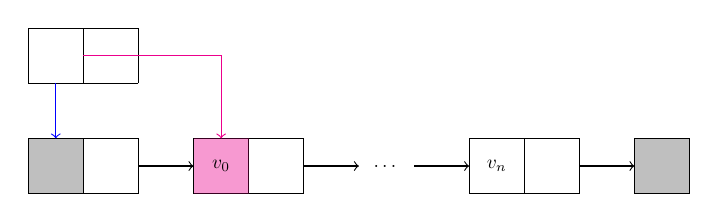
\begin{tikzpicture}[scale=0.7, every node/.style={scale=0.7}]
    \draw (0,0) grid ++(2,1) ;
    \draw [fill=lightgray] (0,0) rectangle ++(1,1) ;
    \draw [->] (2,0.5) -- ++(1,0) ;
    \draw (3,0) grid ++(2,1) ;
    \draw [fill=magenta, opacity=0.4] (3,0) rectangle ++(1,1) ;
    \node at (3.5,0.5) {$v_0$} ;
    \draw [->] (5,0.5) -- ++(1,0) ;
    \node at (6.5,0.5) {\ldots} ;
    \draw [->] (7,0.5) -- ++(1,0) ;
    \draw (8,0) grid ++(2,1) ;
    \node at (8.5,0.5) {$v_n$} ;
    \draw [->] (10,0.5) -- ++(1,0) ;
    \draw [fill=lightgray] (11,0) rectangle ++(1,1) ;
    
    \draw (0,2) grid ++(2,1) ;
    \draw [->, blue] (0.5,2) -- ++(0,-1) ;
    \draw [->, magenta] (1,2.5) -| ++(2.5,-1.5) ;
\end{tikzpicture}
\vfill
\begin{tabular}{c}
        $\mathrm{queue \mathhyphen model}\ t\ [v_0, \cdots, v_n]$
    \\
        $\Downarrow$
    \\
        $\mathrm{queue \mathhyphen model}\ t\ [v_1, \cdots, v_n]$
\end{tabular}
\end{adjustwidth}
\end{frame}

% ---------------------------------------------------------

\begin{frame}[fragile]{Optimized \OCaml~5 implementation --- first try}
\small
\begin{minted}{ocaml}
type ('a, _) node =
  | Nil : ('a, [> `Nil]) node
  | Next : {
      mutable next: ('a, [`Nil | `Next]) node ;
      mutable value: 'a ;
    } -> 
    ('a, [> `Next]) node

external node_as_atomic :
  ('a, [`Next]) node ->
  ('a, [`Nil | `Next]) node Atomic.t
= "%identity"

let push t v =
  ...
  if Atomic.compare_and_set (node_as_atomic back) Nil node
  then ...
  else ...
\end{minted}
\end{frame}

% ---------------------------------------------------------

\begin{frame}{A new hope}
\centering
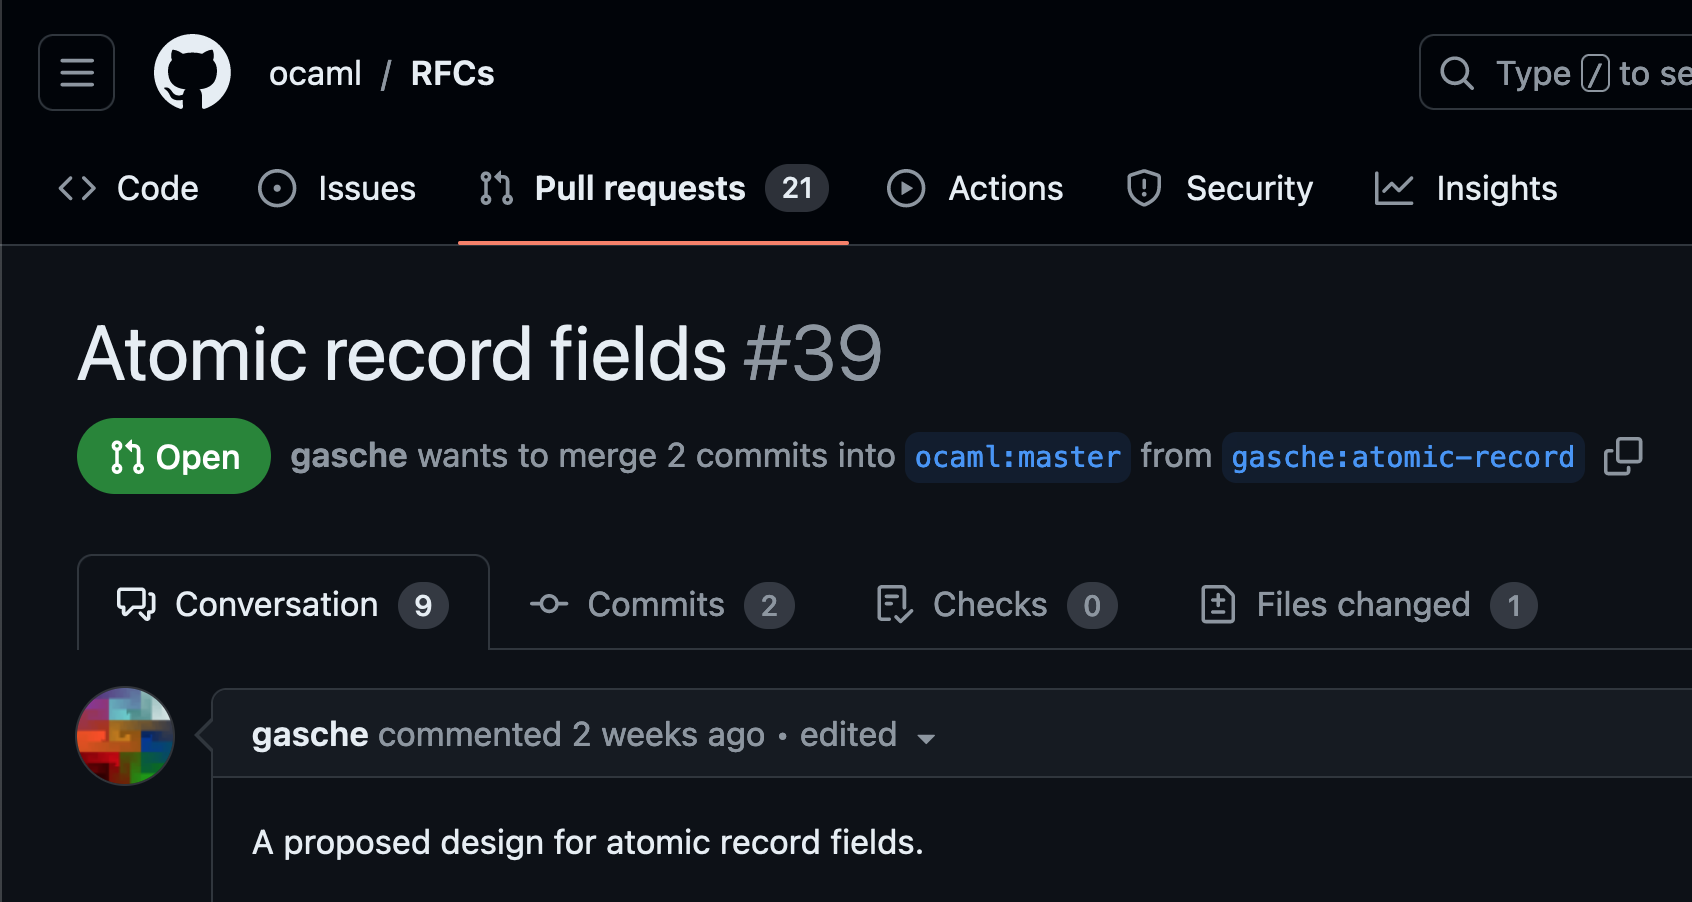
\includegraphics[scale=0.35]{images/rfc.png}
\vfill
(no modification of the \OCaml~5 memory model)
\end{frame}

% ---------------------------------------------------------

\begin{frame}[fragile]{Optimized \OCaml~5 implementation --- second try}
\begin{minted}{ocaml}
type ('a, _) node =
  | Nil : ('a, [> `Nil]) node
  | Next of {
      mutable next: ('a, [`Nil | `Next]) node [@atomic] ;
      mutable value: 'a ;
    } -> 
    ('a, [> `Next]) node

let push t v =
  ...
  if Atomic.Loc.compare_and_set
     [%atomic.field back.next]
     Nil node
  then ...
  else ...
\end{minted}
\end{frame}

% ---------------------------------------------------------

\begin{frame}[fragile]{What about \texttt{is\_empty}?}
\large
\begin{minted}{ocaml}
let is_empty t =
  let Next front = t.front in
  front.next == Nil
\end{minted}
\vfill
\[
  \aspec{
    \mathcolor{cyan}{\mathrm{queue \mathhyphen inv}}\ t\ \iota
  }{
    \mathit{vs}
  }{
    \mathcolor{orange}{\mathrm{queue \mathhyphen model}}\ t\ \mathit{vs}
  }{
    \texttt{queue\_is\_empty}\ t,\ \uparrow \iota
  }{
    \mathcolor{orange}{\mathrm{queue \mathhyphen model}}\ t\ \mathit{vs}
  }{
    \mathit{vs} \stackrel{?}{=} \texttt{[]}
  }{
    \iTrue
  }
\]
\end{frame}

% ---------------------------------------------------------

\begin{frame}{\texttt{is\_empty} (potentially external) linearization}
\begin{adjustwidth}{-1em}{-1em}
\centering
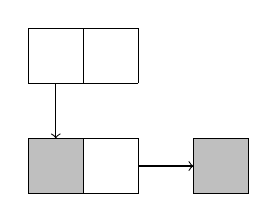
\begin{tikzpicture}[scale=0.7, every node/.style={scale=0.7}]
    \draw (0,0) grid ++(2,1) ;
    \draw [fill=lightgray] (0,0) rectangle ++(1,1) ;
    \draw [->] (2,0.5) -- ++(1,0) ;
    \draw [fill=lightgray] (3,0) rectangle ++(1,1) ;
    
    \draw (0,2) grid ++(2,1) ;
    \draw [->] (0.5,2) -- ++(0,-1) ;
\end{tikzpicture}
\[
    [v_0, \cdots, v_n] = []
\]
\vfill
\hrule
\vfill
\[
    [v_0, \cdots, v_n] \neq []
\]
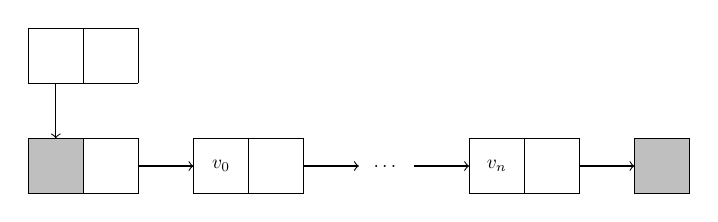
\begin{tikzpicture}[scale=0.7, every node/.style={scale=0.7}]
    \draw (0,0) grid ++(2,1) ;
    \draw [fill=lightgray] (0,0) rectangle ++(1,1) ;
    \draw [->] (2,0.5) -- ++(1,0) ;
    \draw (3,0) grid ++(2,1) ;
    \node at (3.5,0.5) {$v_0$} ;
    \draw [->] (5,0.5) -- ++(1,0) ;
    \node at (6.5,0.5) {\ldots} ;
    \draw [->] (7,0.5) -- ++(1,0) ;
    \draw (8,0) grid ++(2,1) ;
    \node at (8.5,0.5) {$v_n$} ;
    \draw [->] (10,0.5) -- ++(1,0) ;
    \draw [fill=lightgray] (11,0) rectangle ++(1,1) ;
    
    \draw (0,2) grid ++(2,1) ;
    \draw [->] (0.5,2) -- ++(0,-1) ;
\end{tikzpicture}
\end{adjustwidth}
\end{frame}

% ---------------------------------------------------------

\begin{frame}[fragile]{\Iris invariant}
\begin{adjustwidth}{-1.5em}{-1.5em}
\small
\begin{minted}{coq}
Definition queue_inv l γ ι : iProp Σ :=
  ∃ hist past front nodes back vs waiters,
  
  ⌜hist = past ++ front :: nodes⌝ ∗
  ⌜back ∈ hist⌝ ∗
  
  l.[front] ↦ #front ∗
  l.[back] ↦ #back ∗
  
  queue_front_auth γ (length past) ∗
  
  queue_history_auth γ hist ∗
  xchain_model hist () ∗
  
  queue_model₂ γ vs ∗
  ([∗ list] node; v ∈ nodes; vs, node.[xchain_data] ↦ v) ∗
  
  queue_waiters_auth γ waiters ∗
  ([∗ map] waiter ↦ i ∈ waiters, queue_waiter γ ι past waiter i).
\end{minted}
\end{adjustwidth}
\end{frame}

% ---------------------------------------------------------

\begin{frame}{What more?}
\large
\begin{itemize}
    \item Multi-producer \emph{single-consumer} queue.
    \item Multi-producer multi-consumer \emph{bounded} queue.
    \item More advanced queues derived from Michael-Scott?
    \item \href{https://iris-project.org/workshop-2023/slides/moine.pdf}{Space complexity} by Alexandre Moine.
\end{itemize}
\end{frame}